% !TeX spellcheck = de_CH
%%%%%%%%%%%%%%%%%%%%%%%%%%%%%%%%%%%%%%%%%%%%%%%%%%%%%%%%%%%%%%%%%
%  _____   ____  _____                                          %
% |_   _| /  __||  __ \    Institute of Computitional Physics   %
%   | |  |  /   | |__) |   Zuercher Hochschule Winterthur       %
%   | |  | (    |  ___/    (University of Applied Sciences)     %
%  _| |_ |  \__ | |        8401 Winterthur, Switzerland         %
% |_____| \____||_|                                             %
%%%%%%%%%%%%%%%%%%%%%%%%%%%%%%%%%%%%%%%%%%%%%%%%%%%%%%%%%%%%%%%%%
%
% Project     : Konzept BA Welti Keller
% Title       : 
% File        : hardware.tex Rev. 00
% Date        : 15.09.2014
% Author      : Tobias Welti
%
%%%%%%%%%%%%%%%%%%%%%%%%%%%%%%%%%%%%%%%%%%%%%%%%%%%%%%%%%%%%%%%%%

\chapter{Hardware-Konzept}\label{chap.hardware}



\section{Hardware-Architektur}\label{sec.hw_arch}

Anhand der funktionalen Vorgaben für die Messstation werden der Datenlogger, die Sensoreinheit und das Bussytem im folgenden genauer spezifiziert und die Komponenten ausgewählt.

\subsection{Datenlogger}
Der Datenlogger sammelt die Daten der Sensoreinheiten über das Bussystem ein und speichert sie ab. Dafür benötigt er das Bussystem, einen Mikroprozessor, internen Speicher und ein leicht auswechselbares Speichermedium. Ausserdem soll über eine Schnittstelle ein Computer angeschlossen werden können, um den Betrieb der Messstation zu steuern.

\subsection{Sensoreinheit}
Die Sensoreinheit benötigt einen Beschleunigungssensor, um die Einschläge von Geschiebe zu messen. Über einen Analog-Digital-Wandler (ADC) werden die Messsignale digitalisiert. Die gemessenen Signale werden von einem Mikroprozessor verarbeitet, im internen Speicher zwischengespeichert und über das Bussystem an den Datenlogger übertragen.

\subsection{Bussystem}
Das Bussystem muss die Daten und Befehle zwischen Datenlogger und Sensoreinheiten übertragen. Die Reichweite des Bussystems muss genügen, um alle Komponenten der Messinstallation zu verbinden. Die Datenbandbreite muss die Übertragung der Messresultate aller Sensoren erlauben.


\section{Komponentenauswahl}

\subsection{Mikroprozessor}
Bei der Auswahl des Mikroprozessors werden folgende Kriterien berücksichtigt:

\begin{itemize}
\item Rechenleistung genügend für allfällige zusätzliche Anforderungen.
\item Analog-Digital-Wandler mit genügender Abtastrate und Auflösung.
\item Digitaler Signal Prozessor integriert für die Verarbeitung der Messdaten.
\item Ein-/Ausgänge für das Bussystem.
\item Ein-/Ausgänge für den externen Speicher.
\item möglichst geringer Stromverbrauch.
\end{itemize}

\todo{Tabelle verschiedener uCs zum Vergleich}

\subsection{Bus-System}
Anhand folgender Kriterien wurde ein Bussystem ausgewählt:

\begin{itemize}
\item Übertragungsbandbreite genügend für fortlaufende Übertragung von Rohdaten einer Sensoreinheit.
\item Reichweite mindestens 20 Meter.
\item Robust gegenüber äusseren Einflüssen.
\item Mindestens zwanzig Busteilnehmer möglich.
\end{itemize}

\begin{table}
\begin{tabular}{|l|l|l|l|l|}
\hline  & \textbf{Bitrate}      & \textbf{Distanz} & \textbf{Clients} & \textbf{Besonderheiten}\\ 
\hline \textbf{CAN} & \begin{minipage}{2cm}
1 MBit/s\\ 125 kBit/s
\end{minipage} & \begin{minipage}{1.5cm}40 m\\500 m\end{minipage} & > 20 & \begin{minipage}{6cm}
\mbox{ }\\+ Collision Detection (CD) umgehen mit Polling durch Master.\\
+ Bei synchronem CAN wird CD durch ID gelöst.\\
+ CAN Controller sendet Interrupt Request bei erhaltener Nachricht.\\
\end{minipage} \\ 
\hline \textbf{SPI} & ..100 MBit/s & < 1 m & \begin{minipage}{1cm}
slave select
\end{minipage} & \begin{minipage}{6cm}
\mbox{ }\\- Pro Client eine Slave Select Leitung\\
- Daisy Chain $\Rightarrow $alle MC beschäftigt.\\
- Bei Ausfall eines MC ganzer Bus unterbrochen.\\
\end{minipage} \\ 
\hline \textbf{RS485} & \begin{minipage}{2cm}
35 MBit/s\\100 kBit/s
\end{minipage} & \begin{minipage}{1.5cm}
10 m\\1200 m
\end{minipage} & >32 & \begin{minipage}{6cm}
\mbox{ }\\- Master am besten in der Mitte des Bus $\Rightarrow$ ungünstig.\\
- Braucht 2..4 Drähte (bei Full Duplex)\\
- braucht pull-up und pull-down Widerstände $\Rightarrow$ mehr Leistungsaufnahme.\\
\end{minipage} \\ 
\hline \textbf{Ethernet} & 100 MBit/s & 100 m & > 20 & \begin{minipage}{6cm}
\mbox{ }\\+ Stromversorgung bei Power over Ethernet (PoE) integriert.\\
- kein Bus sondern allenfalls Daisychain.\\
- bei Daisychain kein PoE möglich.\\
\end{minipage} \\ 
\hline \textbf{Feldbus} &  &  &  & \begin{minipage}{6cm}
\mbox{ }\\ist eine Familie von Bussen, z.B. CAN-Bus\\
\end{minipage} \\ 
\hline \textbf{I2C} & 0.4..5 Mbit/s & wenige Meter & < 20 & \begin{minipage}{6cm}
\mbox{ }\\nur für kurze Distanzen, Bitrate nimmt rasch ab.\\
\end{minipage}\\
\hline 
\end{tabular}
\caption{Entscheidungsmatrix für die Auswahl des Bussystems.}
\label{table.bussystem}
\end{table} 

In Tabelle \ref{table.bussystem} sind die Eigenschaften diverser Bussysteme aufgeführt.

\paragraph{Kommentare}
SPI und I2C sind nur für kurze Distanzen geeignet und sind deshalb keine Option.
Die Verwendung von Ethernet zur Datenübertragung würde zwei Schnittstellen auf jeder Sensoreinheit voraussetzen, um die Sensoren hintereinander zusammenzuhängen (Daisychain). Jedes Paket müsste vom Microcontroller weitergeleitet werden, wenn es für einen anderen Empfänger bestimmt ist. Dies führte zu einer zusätzlichen Belastung der Microcontroller. Stromversorgung über Ethernet ist mit PowerOverEthernet (PoE) zwar möglich, erfordert aber spezielle Geräte zur Speisung über den Stecker des Datenkabels. Dies verunmöglicht eine Daisychain mit PoE, neben dem Datenkabel wäre noch ein Kabel für die Stromversorgung notwendig.

\paragraph{Entscheidung}
CAN-Bus erfüllt alle Kriterien und erlaubt es, den Busmaster am Ende des Bus zu platzieren. Dies ist ein Vorteil gegenüber RS485, wo der Master in der Mitte platziert werden sollte. Für CAN-Bus sind Bus-Treiber (Transceiver) erhältlich, die mit hohen Spannungen umgehen können, was das Bussystem robuster gegenüber Umwelteinflüssen macht. 



\subsection{Speichermedium}
\paragraph{Kriterien} Das externe Speichermedium soll möglichst klein sein, wenig Stromverbrauch haben und einfach auswechselbar sein. Bei Inaktivität sollte das Medium wenn möglich keinen Strom verbrauchen. Für einen mehrwöchigen unabhängigen Betrieb einer Messstation muss genügend Speicherkapazität bereitgestellt werden.

\paragraph{Datenmenge} Pro Sensor werden bei hohem Geschiebeaufkommen maximal hundert Ereignisse pro Sekunde erwartet. Ein solches Geschiebeaufkommen stellt jedoch die Ausnahme dar. Ein Ereignis benötigt je nach verlangtem Detailgrad und Dauer des Ereignisses 10..90 Byte Speicherplatz. Für den normalen Betriebsmodus werden 50 Byte/Ereignis gerechnet, bei 5 Ereignissen pro Sekunde. Damit ergibt sich eine Datenrate von 250 Byte/s, die es pro Sensor abzuspeichern gilt. Mit zehn Sensoren im Einsatz müssen 2.5 kByte/s gespeichert werden. 

\paragraph{Unabhängige Betriebsdauer} Pro Gigabyte Speicherplatz können 111 Stunden Daten für zehn Sensoren gespeichert werden. Bei hohem Geschiebeaufkommen mit zwanzig mal mehr Ereignissen bleiben immer noch 5 Stunden Aufzeichnungszeit pro Gigabyte. Begnügt man sich mit weniger Details, reichen fallen pro Sensor in zehn Sekunden rund 400 Byte Daten an. Bei dieser Datenrate reicht ein Gigabyte für rund 700 Stunden. Auch bei hohem Geschiebeaufkommen kann die Anlage mehrere Tage an Daten speichern. 

\paragraph{Kapazität} Heute sind Speichermedien mit Kapazitäten bis über 128 GB erhältlich, so dass die Detailrate kein entscheidendes Kriterium mehr darstellt.

\paragraph{Datentransfer} Für den Transfer der Daten aus dem Datenlogger auf einen Computer gibt es grundsätzlich zwei Varianten. Entweder man liest die Daten über eine Schnittstelle auf den Computer aus, oder man tauscht das Speichermedium aus. Das Auslesen via Schnittstelle benötigt zusätzlich Strom, das Wechseln des Speichermediums setzt einen mehr oder weniger komfortablen und trotzdem wasserdichten Zugang zum Medium voraus. Da heute Speichermedien mit kleinem Platzbedarf erhältlich sind, könnte ein solcher Zugang recht einfach mit einem Schraubverschluss realisiert werden.

\paragraph{Vergleich} In Tabelle \ref{table.speichermedium} werden verschiedene Speichermedien miteinander verglichen. In der Spalte 'Breite' ist aufgelistet, wie gross eine Öffnung mindestens sein muss, um das Speichermedium wechseln zu können. 'Pins' gibt an, wie viele Leitungen für den Anschluss des Mediums am Microcontroller nötig sind. Der Stromverbrauch in Klammern ist für den Standby-Modus des Speichermediums.

\begin{table}
\begin{tabular}{|l|l|l|l|l|}
	\hline
	                      & \textbf{Breite} & \textbf{Pins} & \textbf{Stromverbrauch} & \textbf{Bemerkungen}        \\ \hline
	\textbf{SD-Card}      & 24 mm           & 9             & 20..100 mA (0.2 mA)     & 4 bit breiter serieller Bus \\ \hline
	\textbf{CompactFlash} & 43 mm           & 50            & max. 70 mA (k.A.)       & paralleler Bus              \\ \hline
	\textbf{USB-Stick}    & min. 12 mm      & 4             & typ. 70 mA (k.A.) &  \\ \hline
\end{tabular} 
\caption{Entscheidungsmatrix zur Auswahl des Speichermediums.}
\label{table.speichermedium}
\end{table} 

\todo{Referenzen (wiki) in Tabelle \ref{table.speichermedium}}


\paragraph{Entscheid} 

\subsection{Sensor}


\subsection{Schnittstelle}




\section{Komponenten}

\subsection{Cortex M4 Mikroprozessor}

\subsubsection{Flash Speicher}

\subsubsection{SDRAM}


\subsection{Beschleunigungs-Sensor}

\subsection{CAN Bus}

\subsubsection{CAN Transceiver}


\subsection{SD Karte}

\subsection{UART Schnittstelle}

\section{Datenlogger}

\begin{figure}[H]
	\centering
		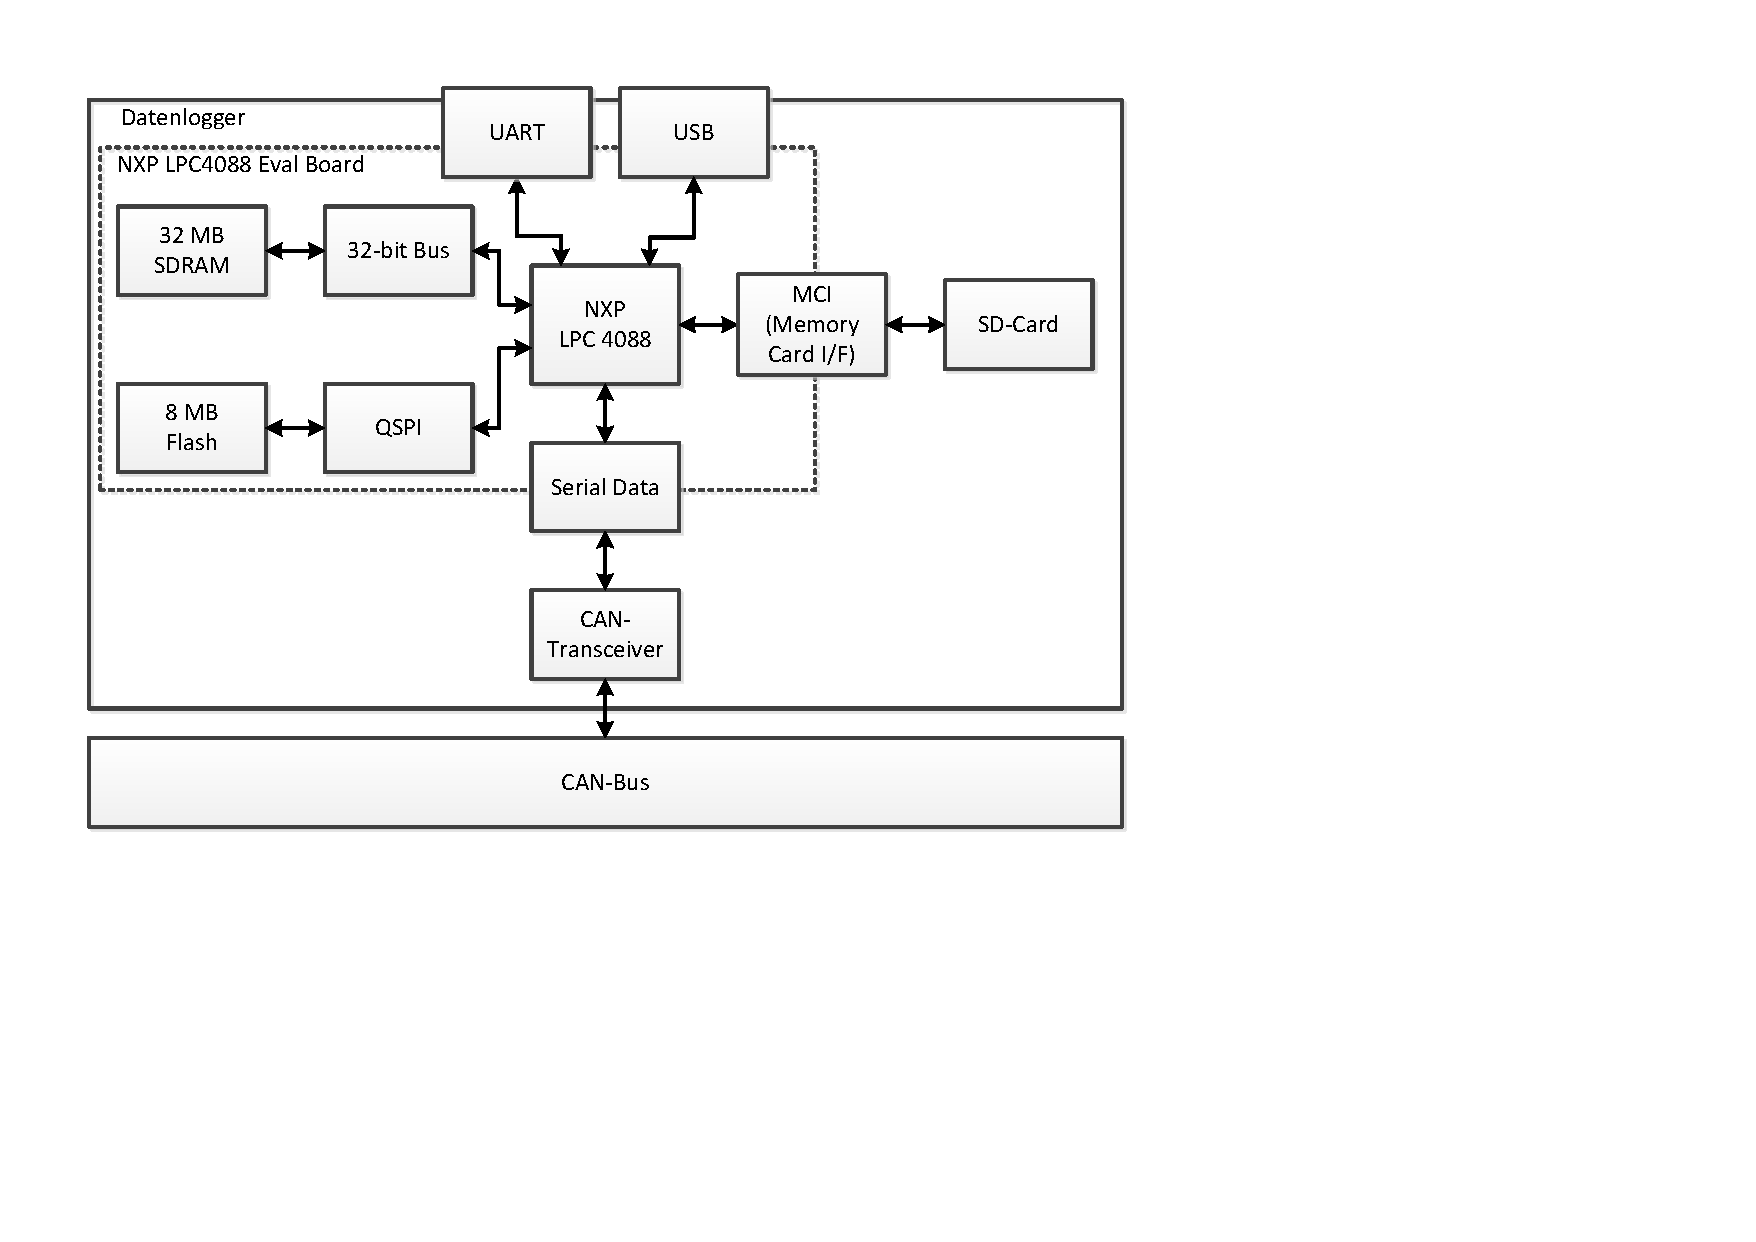
\includegraphics[width=0.8\textwidth]{images/visio/hardware_logger.pdf}
	\caption{Schematischer Hardware-Aufbau des Datenloggers.}
	\label{fig.hw_logger}
\end{figure}



\section{Sensoreinheit}

\begin{figure}[H]
	\centering
		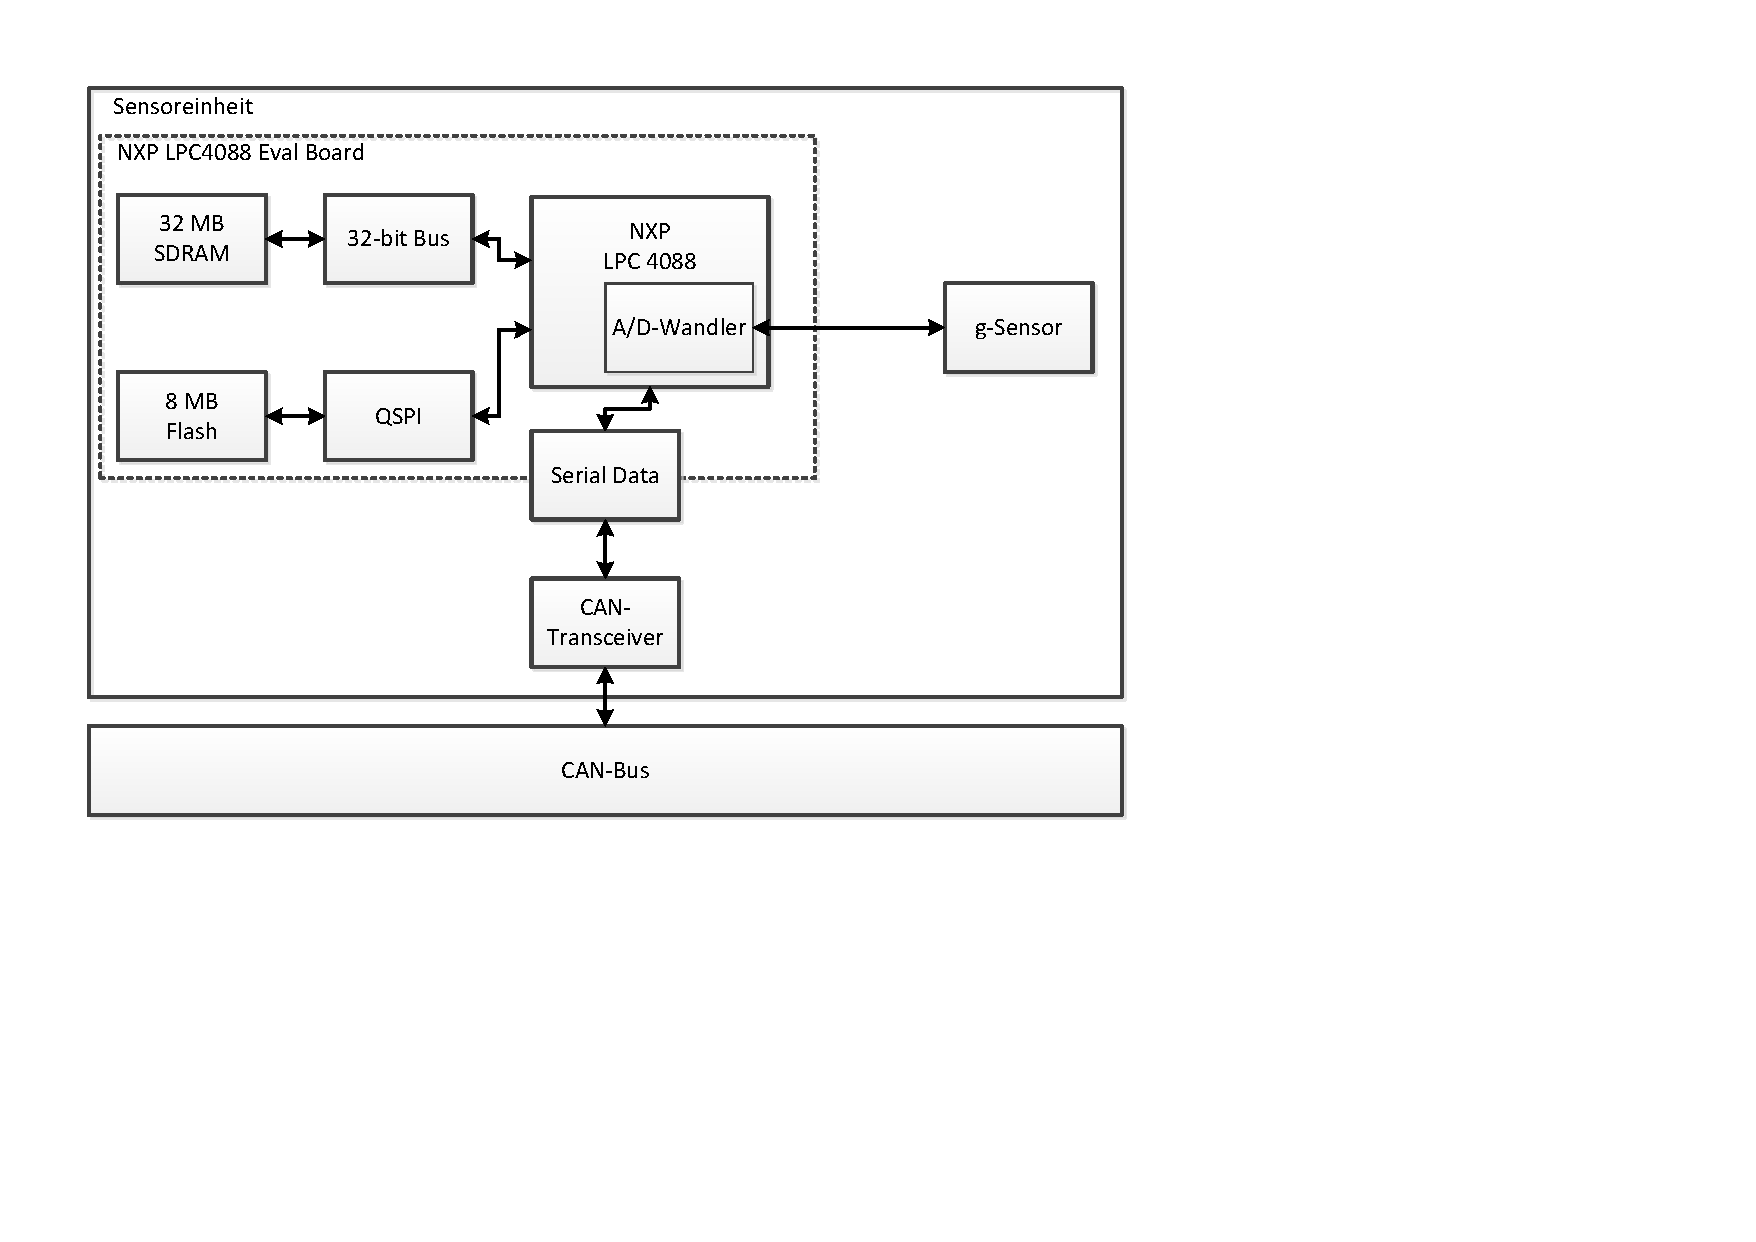
\includegraphics[width=0.8\textwidth]{images/visio/hardware_sensor.pdf}
	\caption{Schematischer Hardware-Aufbau der Sensoreinheit.}
	\label{fig.hw_sensor}
\end{figure}


